% Created by tikzDevice version 0.12.6 on 2024-04-08 15:44:17
% !TEX encoding = UTF-8 Unicode
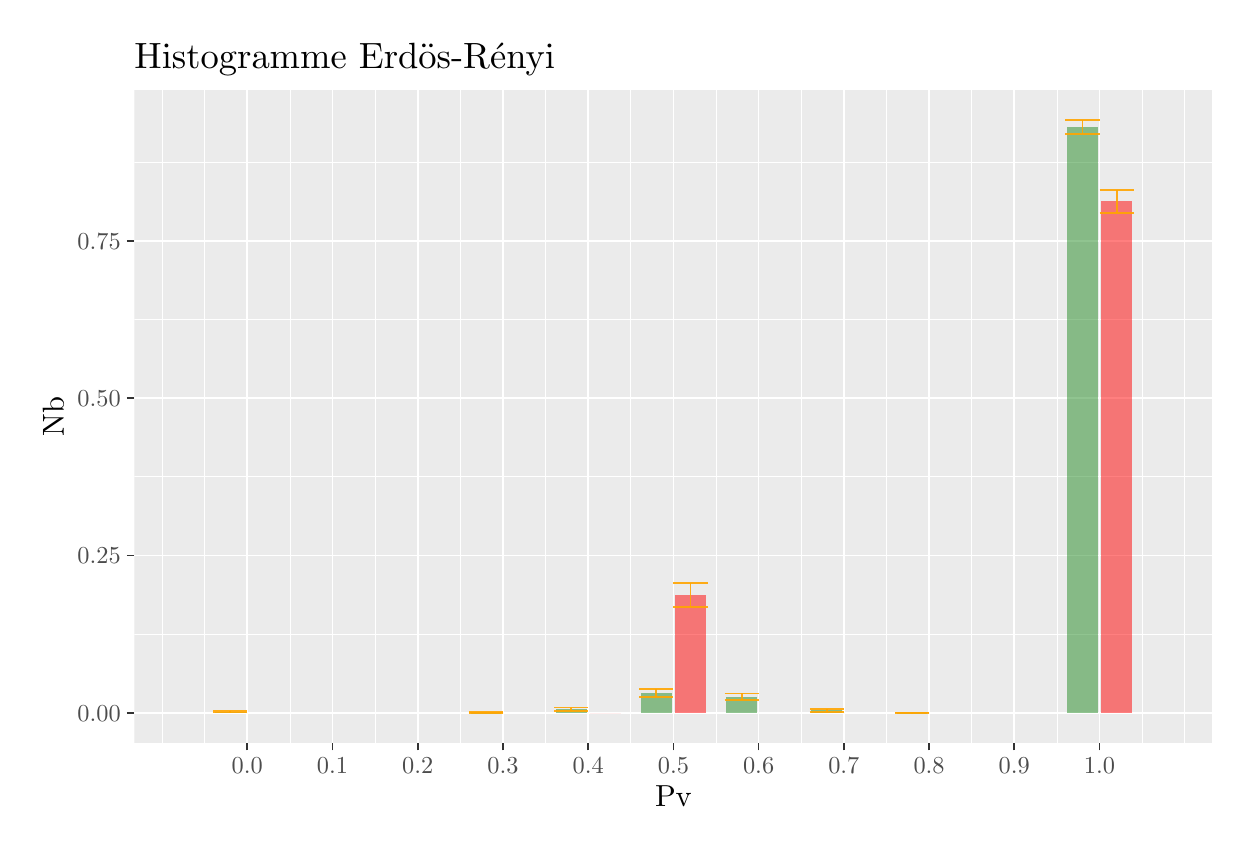
\begin{tikzpicture}[x=1pt,y=1pt]
\definecolor{fillColor}{RGB}{255,255,255}
\path[use as bounding box,fill=fillColor,fill opacity=0.00] (0,0) rectangle (433.62,289.08);
\begin{scope}
\path[clip] (  0.00,  0.00) rectangle (433.62,289.08);
\definecolor{drawColor}{RGB}{255,255,255}
\definecolor{fillColor}{RGB}{255,255,255}

\path[draw=drawColor,line width= 0.6pt,line join=round,line cap=round,fill=fillColor] (  0.00,  0.00) rectangle (433.62,289.08);
\end{scope}
\begin{scope}
\path[clip] ( 38.56, 30.69) rectangle (428.12,266.42);
\definecolor{fillColor}{gray}{0.92}

\path[fill=fillColor] ( 38.56, 30.69) rectangle (428.12,266.42);
\definecolor{drawColor}{RGB}{255,255,255}

\path[draw=drawColor,line width= 0.3pt,line join=round] ( 38.56, 69.89) --
	(428.12, 69.89);

\path[draw=drawColor,line width= 0.3pt,line join=round] ( 38.56,126.75) --
	(428.12,126.75);

\path[draw=drawColor,line width= 0.3pt,line join=round] ( 38.56,183.61) --
	(428.12,183.61);

\path[draw=drawColor,line width= 0.3pt,line join=round] ( 38.56,240.48) --
	(428.12,240.48);

\path[draw=drawColor,line width= 0.3pt,line join=round] ( 48.56, 30.69) --
	( 48.56,266.42);

\path[draw=drawColor,line width= 0.3pt,line join=round] ( 63.96, 30.69) --
	( 63.96,266.42);

\path[draw=drawColor,line width= 0.3pt,line join=round] ( 94.76, 30.69) --
	( 94.76,266.42);

\path[draw=drawColor,line width= 0.3pt,line join=round] (125.55, 30.69) --
	(125.55,266.42);

\path[draw=drawColor,line width= 0.3pt,line join=round] (156.35, 30.69) --
	(156.35,266.42);

\path[draw=drawColor,line width= 0.3pt,line join=round] (187.14, 30.69) --
	(187.14,266.42);

\path[draw=drawColor,line width= 0.3pt,line join=round] (217.94, 30.69) --
	(217.94,266.42);

\path[draw=drawColor,line width= 0.3pt,line join=round] (248.74, 30.69) --
	(248.74,266.42);

\path[draw=drawColor,line width= 0.3pt,line join=round] (279.53, 30.69) --
	(279.53,266.42);

\path[draw=drawColor,line width= 0.3pt,line join=round] (310.33, 30.69) --
	(310.33,266.42);

\path[draw=drawColor,line width= 0.3pt,line join=round] (341.12, 30.69) --
	(341.12,266.42);

\path[draw=drawColor,line width= 0.3pt,line join=round] (371.92, 30.69) --
	(371.92,266.42);

\path[draw=drawColor,line width= 0.3pt,line join=round] (402.71, 30.69) --
	(402.71,266.42);

\path[draw=drawColor,line width= 0.3pt,line join=round] (418.11, 30.69) --
	(418.11,266.42);

\path[draw=drawColor,line width= 0.6pt,line join=round] ( 38.56, 41.46) --
	(428.12, 41.46);

\path[draw=drawColor,line width= 0.6pt,line join=round] ( 38.56, 98.32) --
	(428.12, 98.32);

\path[draw=drawColor,line width= 0.6pt,line join=round] ( 38.56,155.18) --
	(428.12,155.18);

\path[draw=drawColor,line width= 0.6pt,line join=round] ( 38.56,212.05) --
	(428.12,212.05);

\path[draw=drawColor,line width= 0.6pt,line join=round] ( 79.36, 30.69) --
	( 79.36,266.42);

\path[draw=drawColor,line width= 0.6pt,line join=round] (110.15, 30.69) --
	(110.15,266.42);

\path[draw=drawColor,line width= 0.6pt,line join=round] (140.95, 30.69) --
	(140.95,266.42);

\path[draw=drawColor,line width= 0.6pt,line join=round] (171.75, 30.69) --
	(171.75,266.42);

\path[draw=drawColor,line width= 0.6pt,line join=round] (202.54, 30.69) --
	(202.54,266.42);

\path[draw=drawColor,line width= 0.6pt,line join=round] (233.34, 30.69) --
	(233.34,266.42);

\path[draw=drawColor,line width= 0.6pt,line join=round] (264.13, 30.69) --
	(264.13,266.42);

\path[draw=drawColor,line width= 0.6pt,line join=round] (294.93, 30.69) --
	(294.93,266.42);

\path[draw=drawColor,line width= 0.6pt,line join=round] (325.72, 30.69) --
	(325.72,266.42);

\path[draw=drawColor,line width= 0.6pt,line join=round] (356.52, 30.69) --
	(356.52,266.42);

\path[draw=drawColor,line width= 0.6pt,line join=round] (387.32, 30.69) --
	(387.32,266.42);
\definecolor{fillColor}{RGB}{34,139,34}

\path[fill=fillColor,fill opacity=0.50] ( 67.66, 41.46) rectangle ( 78.74, 41.90);

\path[fill=fillColor,fill opacity=0.50] (160.04, 41.46) rectangle (171.13, 41.56);

\path[fill=fillColor,fill opacity=0.50] (190.84, 41.46) rectangle (201.93, 42.87);

\path[fill=fillColor,fill opacity=0.50] (221.64, 41.46) rectangle (232.72, 48.54);

\path[fill=fillColor,fill opacity=0.50] (252.43, 41.46) rectangle (263.52, 47.27);

\path[fill=fillColor,fill opacity=0.50] (283.23, 41.46) rectangle (294.31, 42.36);

\path[fill=fillColor,fill opacity=0.50] (314.02, 41.46) rectangle (325.11, 41.51);

\path[fill=fillColor,fill opacity=0.50] (375.61, 41.46) rectangle (386.70,253.10);
\definecolor{fillColor}{RGB}{255,0,0}

\path[fill=fillColor,fill opacity=0.50] (203.16, 41.46) rectangle (214.24, 41.46);

\path[fill=fillColor,fill opacity=0.50] (233.95, 41.46) rectangle (245.04, 84.08);

\path[fill=fillColor,fill opacity=0.50] (387.93, 41.46) rectangle (399.02,226.27);
\definecolor{drawColor}{RGB}{255,165,0}

\path[draw=drawColor,draw opacity=0.90,line width= 0.7pt,line join=round] ( 67.04, 42.20) --
	( 79.36, 42.20);

\path[draw=drawColor,draw opacity=0.90,line width= 0.7pt,line join=round] ( 73.20, 42.20) --
	( 73.20, 41.61);

\path[draw=drawColor,draw opacity=0.90,line width= 0.7pt,line join=round] ( 67.04, 41.61) --
	( 79.36, 41.61);

\path[draw=drawColor,draw opacity=0.90,line width= 0.7pt,line join=round] (159.43, 41.72) --
	(171.75, 41.72);

\path[draw=drawColor,draw opacity=0.90,line width= 0.7pt,line join=round] (165.59, 41.72) --
	(165.59, 41.41);

\path[draw=drawColor,draw opacity=0.90,line width= 0.7pt,line join=round] (159.43, 41.41) --
	(171.75, 41.41);

\path[draw=drawColor,draw opacity=0.90,line width= 0.7pt,line join=round] (190.22, 43.42) --
	(202.54, 43.42);

\path[draw=drawColor,draw opacity=0.90,line width= 0.7pt,line join=round] (196.38, 43.42) --
	(196.38, 42.32);

\path[draw=drawColor,draw opacity=0.90,line width= 0.7pt,line join=round] (190.22, 42.32) --
	(202.54, 42.32);

\path[draw=drawColor,draw opacity=0.90,line width= 0.7pt,line join=round] (221.02, 50.00) --
	(233.34, 50.00);

\path[draw=drawColor,draw opacity=0.90,line width= 0.7pt,line join=round] (227.18, 50.00) --
	(227.18, 47.08);

\path[draw=drawColor,draw opacity=0.90,line width= 0.7pt,line join=round] (221.02, 47.08) --
	(233.34, 47.08);

\path[draw=drawColor,draw opacity=0.90,line width= 0.7pt,line join=round] (251.81, 48.49) --
	(264.13, 48.49);

\path[draw=drawColor,draw opacity=0.90,line width= 0.7pt,line join=round] (257.97, 48.49) --
	(257.97, 46.04);

\path[draw=drawColor,draw opacity=0.90,line width= 0.7pt,line join=round] (251.81, 46.04) --
	(264.13, 46.04);

\path[draw=drawColor,draw opacity=0.90,line width= 0.7pt,line join=round] (282.61, 42.80) --
	(294.93, 42.80);

\path[draw=drawColor,draw opacity=0.90,line width= 0.7pt,line join=round] (288.77, 42.80) --
	(288.77, 41.91);

\path[draw=drawColor,draw opacity=0.90,line width= 0.7pt,line join=round] (282.61, 41.91) --
	(294.93, 41.91);

\path[draw=drawColor,draw opacity=0.90,line width= 0.7pt,line join=round] (313.41, 41.61) --
	(325.72, 41.61);

\path[draw=drawColor,draw opacity=0.90,line width= 0.7pt,line join=round] (319.57, 41.61) --
	(319.57, 41.40);

\path[draw=drawColor,draw opacity=0.90,line width= 0.7pt,line join=round] (313.41, 41.40) --
	(325.72, 41.40);

\path[draw=drawColor,draw opacity=0.90,line width= 0.7pt,line join=round] (375.00,255.71) --
	(387.32,255.71);

\path[draw=drawColor,draw opacity=0.90,line width= 0.7pt,line join=round] (381.16,255.71) --
	(381.16,250.49);

\path[draw=drawColor,draw opacity=0.90,line width= 0.7pt,line join=round] (375.00,250.49) --
	(387.32,250.49);

\path[draw=drawColor,draw opacity=0.90,line width= 0.7pt,line join=round] (233.34, 88.31) --
	(245.66, 88.31);

\path[draw=drawColor,draw opacity=0.90,line width= 0.7pt,line join=round] (239.50, 88.31) --
	(239.50, 79.86);

\path[draw=drawColor,draw opacity=0.90,line width= 0.7pt,line join=round] (233.34, 79.86) --
	(245.66, 79.86);

\path[draw=drawColor,draw opacity=0.90,line width= 0.7pt,line join=round] (387.32,230.49) --
	(399.63,230.49);

\path[draw=drawColor,draw opacity=0.90,line width= 0.7pt,line join=round] (393.47,230.49) --
	(393.47,222.06);

\path[draw=drawColor,draw opacity=0.90,line width= 0.7pt,line join=round] (387.32,222.06) --
	(399.63,222.06);
\end{scope}
\begin{scope}
\path[clip] (  0.00,  0.00) rectangle (433.62,289.08);
\definecolor{drawColor}{gray}{0.30}

\node[text=drawColor,anchor=base east,inner sep=0pt, outer sep=0pt, scale=  0.88] at ( 33.61, 38.43) {0.00};

\node[text=drawColor,anchor=base east,inner sep=0pt, outer sep=0pt, scale=  0.88] at ( 33.61, 95.29) {0.25};

\node[text=drawColor,anchor=base east,inner sep=0pt, outer sep=0pt, scale=  0.88] at ( 33.61,152.15) {0.50};

\node[text=drawColor,anchor=base east,inner sep=0pt, outer sep=0pt, scale=  0.88] at ( 33.61,209.02) {0.75};
\end{scope}
\begin{scope}
\path[clip] (  0.00,  0.00) rectangle (433.62,289.08);
\definecolor{drawColor}{gray}{0.20}

\path[draw=drawColor,line width= 0.6pt,line join=round] ( 35.81, 41.46) --
	( 38.56, 41.46);

\path[draw=drawColor,line width= 0.6pt,line join=round] ( 35.81, 98.32) --
	( 38.56, 98.32);

\path[draw=drawColor,line width= 0.6pt,line join=round] ( 35.81,155.18) --
	( 38.56,155.18);

\path[draw=drawColor,line width= 0.6pt,line join=round] ( 35.81,212.05) --
	( 38.56,212.05);
\end{scope}
\begin{scope}
\path[clip] (  0.00,  0.00) rectangle (433.62,289.08);
\definecolor{drawColor}{gray}{0.20}

\path[draw=drawColor,line width= 0.6pt,line join=round] ( 79.36, 27.94) --
	( 79.36, 30.69);

\path[draw=drawColor,line width= 0.6pt,line join=round] (110.15, 27.94) --
	(110.15, 30.69);

\path[draw=drawColor,line width= 0.6pt,line join=round] (140.95, 27.94) --
	(140.95, 30.69);

\path[draw=drawColor,line width= 0.6pt,line join=round] (171.75, 27.94) --
	(171.75, 30.69);

\path[draw=drawColor,line width= 0.6pt,line join=round] (202.54, 27.94) --
	(202.54, 30.69);

\path[draw=drawColor,line width= 0.6pt,line join=round] (233.34, 27.94) --
	(233.34, 30.69);

\path[draw=drawColor,line width= 0.6pt,line join=round] (264.13, 27.94) --
	(264.13, 30.69);

\path[draw=drawColor,line width= 0.6pt,line join=round] (294.93, 27.94) --
	(294.93, 30.69);

\path[draw=drawColor,line width= 0.6pt,line join=round] (325.72, 27.94) --
	(325.72, 30.69);

\path[draw=drawColor,line width= 0.6pt,line join=round] (356.52, 27.94) --
	(356.52, 30.69);

\path[draw=drawColor,line width= 0.6pt,line join=round] (387.32, 27.94) --
	(387.32, 30.69);
\end{scope}
\begin{scope}
\path[clip] (  0.00,  0.00) rectangle (433.62,289.08);
\definecolor{drawColor}{gray}{0.30}

\node[text=drawColor,anchor=base,inner sep=0pt, outer sep=0pt, scale=  0.88] at ( 79.36, 19.68) {0.0};

\node[text=drawColor,anchor=base,inner sep=0pt, outer sep=0pt, scale=  0.88] at (110.15, 19.68) {0.1};

\node[text=drawColor,anchor=base,inner sep=0pt, outer sep=0pt, scale=  0.88] at (140.95, 19.68) {0.2};

\node[text=drawColor,anchor=base,inner sep=0pt, outer sep=0pt, scale=  0.88] at (171.75, 19.68) {0.3};

\node[text=drawColor,anchor=base,inner sep=0pt, outer sep=0pt, scale=  0.88] at (202.54, 19.68) {0.4};

\node[text=drawColor,anchor=base,inner sep=0pt, outer sep=0pt, scale=  0.88] at (233.34, 19.68) {0.5};

\node[text=drawColor,anchor=base,inner sep=0pt, outer sep=0pt, scale=  0.88] at (264.13, 19.68) {0.6};

\node[text=drawColor,anchor=base,inner sep=0pt, outer sep=0pt, scale=  0.88] at (294.93, 19.68) {0.7};

\node[text=drawColor,anchor=base,inner sep=0pt, outer sep=0pt, scale=  0.88] at (325.72, 19.68) {0.8};

\node[text=drawColor,anchor=base,inner sep=0pt, outer sep=0pt, scale=  0.88] at (356.52, 19.68) {0.9};

\node[text=drawColor,anchor=base,inner sep=0pt, outer sep=0pt, scale=  0.88] at (387.32, 19.68) {1.0};
\end{scope}
\begin{scope}
\path[clip] (  0.00,  0.00) rectangle (433.62,289.08);
\definecolor{drawColor}{RGB}{0,0,0}

\node[text=drawColor,anchor=base,inner sep=0pt, outer sep=0pt, scale=  1.10] at (233.34,  7.64) {Pv};
\end{scope}
\begin{scope}
\path[clip] (  0.00,  0.00) rectangle (433.62,289.08);
\definecolor{drawColor}{RGB}{0,0,0}

\node[text=drawColor,rotate= 90.00,anchor=base,inner sep=0pt, outer sep=0pt, scale=  1.10] at ( 13.08,148.55) {Nb};
\end{scope}
\begin{scope}
\path[clip] (  0.00,  0.00) rectangle (433.62,289.08);
\definecolor{drawColor}{RGB}{0,0,0}

\node[text=drawColor,anchor=base west,inner sep=0pt, outer sep=0pt, scale=  1.32] at ( 38.56,274.49) {Histogramme Erdös-Rényi};
\end{scope}
\end{tikzpicture}
